% -*- root: ../thesis.tex -*-
%!TEX root = ../thesis.tex
% ******************************* Thesis Chapter 6 ****************************


% ----------------------- paths to graphics ------------------------

% change according to folder and file names
\graphicspath{{7/figures/}}
% ----------------------- contents from here ------------------------
This last published work is a bit different from the rest of the previous chapters.
Instead of focusing on the representation of the model, this works aims at changing the variational distribution representation.
The original motivation behind this work was to answer the question: can we fit a full Gaussian variational distribution to a target distribution while never have to compute any matrix inverses, log determinant or second-order derivative?
The answer resulted in a particle approach: the mean and covariance are replaced by an arbitrary number of points in the variable domain.
Although the method might not be a state-of-the-art approach for variational inference, it brings a lot of insights concerning convergence speed, and accuracy of the given posterior.

\textbf{\underline{Authors:}}\\
Th\'eo Galy-Fajou,$^{1}$, Valerio Perrone,$^{2}$, Manfred Opper$^{1,3}$\\
\small{$^1$TU Berlin, Germany, $^2$Amazon Web Services, $^3$University of Birmingham\\

\textbf{\underline{Details:}}\\
Type: Journal article\\
Submitted: June 2021\\
Accepted: July 2021\\
URL: \url{https://www.mdpi.com/1099-4300/23/8/990}\\
Journal: Entropy (Special edition on Approximate Bayesian Inference)\\
License: Creative Commons Attribution (CC BY 4.0)\\

% ----------------------- contents from here ------------------------
\newpage
\underline{\textbf{Contributions:}}\\
For an explanation of the terms see the \href{https://mdpi-res.com/data/contributor-role-instruction.pdf}{Contributor Roles Taxonomy} (CReditT)\\
\begin{center}
\begin{tabular}{c|c|c|c|}
    & T.G-F. & V.P. & M.O.\\\hline
    \textbf{Conceptualization} & \checkmark &  & \checkmark\\
    \textbf{Methodology} & \checkmark & \checkmark & \checkmark \\
    \textbf{Formal Analysis} & \checkmark & & \\
    \textbf{Software} & \checkmark & & \\
    \textbf{Investigation} & \checkmark & & \\
    \textbf{Writing - Original Draft} & \checkmark & \checkmark & \checkmark\\
    \textbf{Writing - Review \& Editing} & \checkmark & \checkmark & \checkmark\\
    \textbf{Supervision} & & & \checkmark\\
    \textbf{Funding Acquisition} & & & \checkmark
\end{tabular}
\end{center}
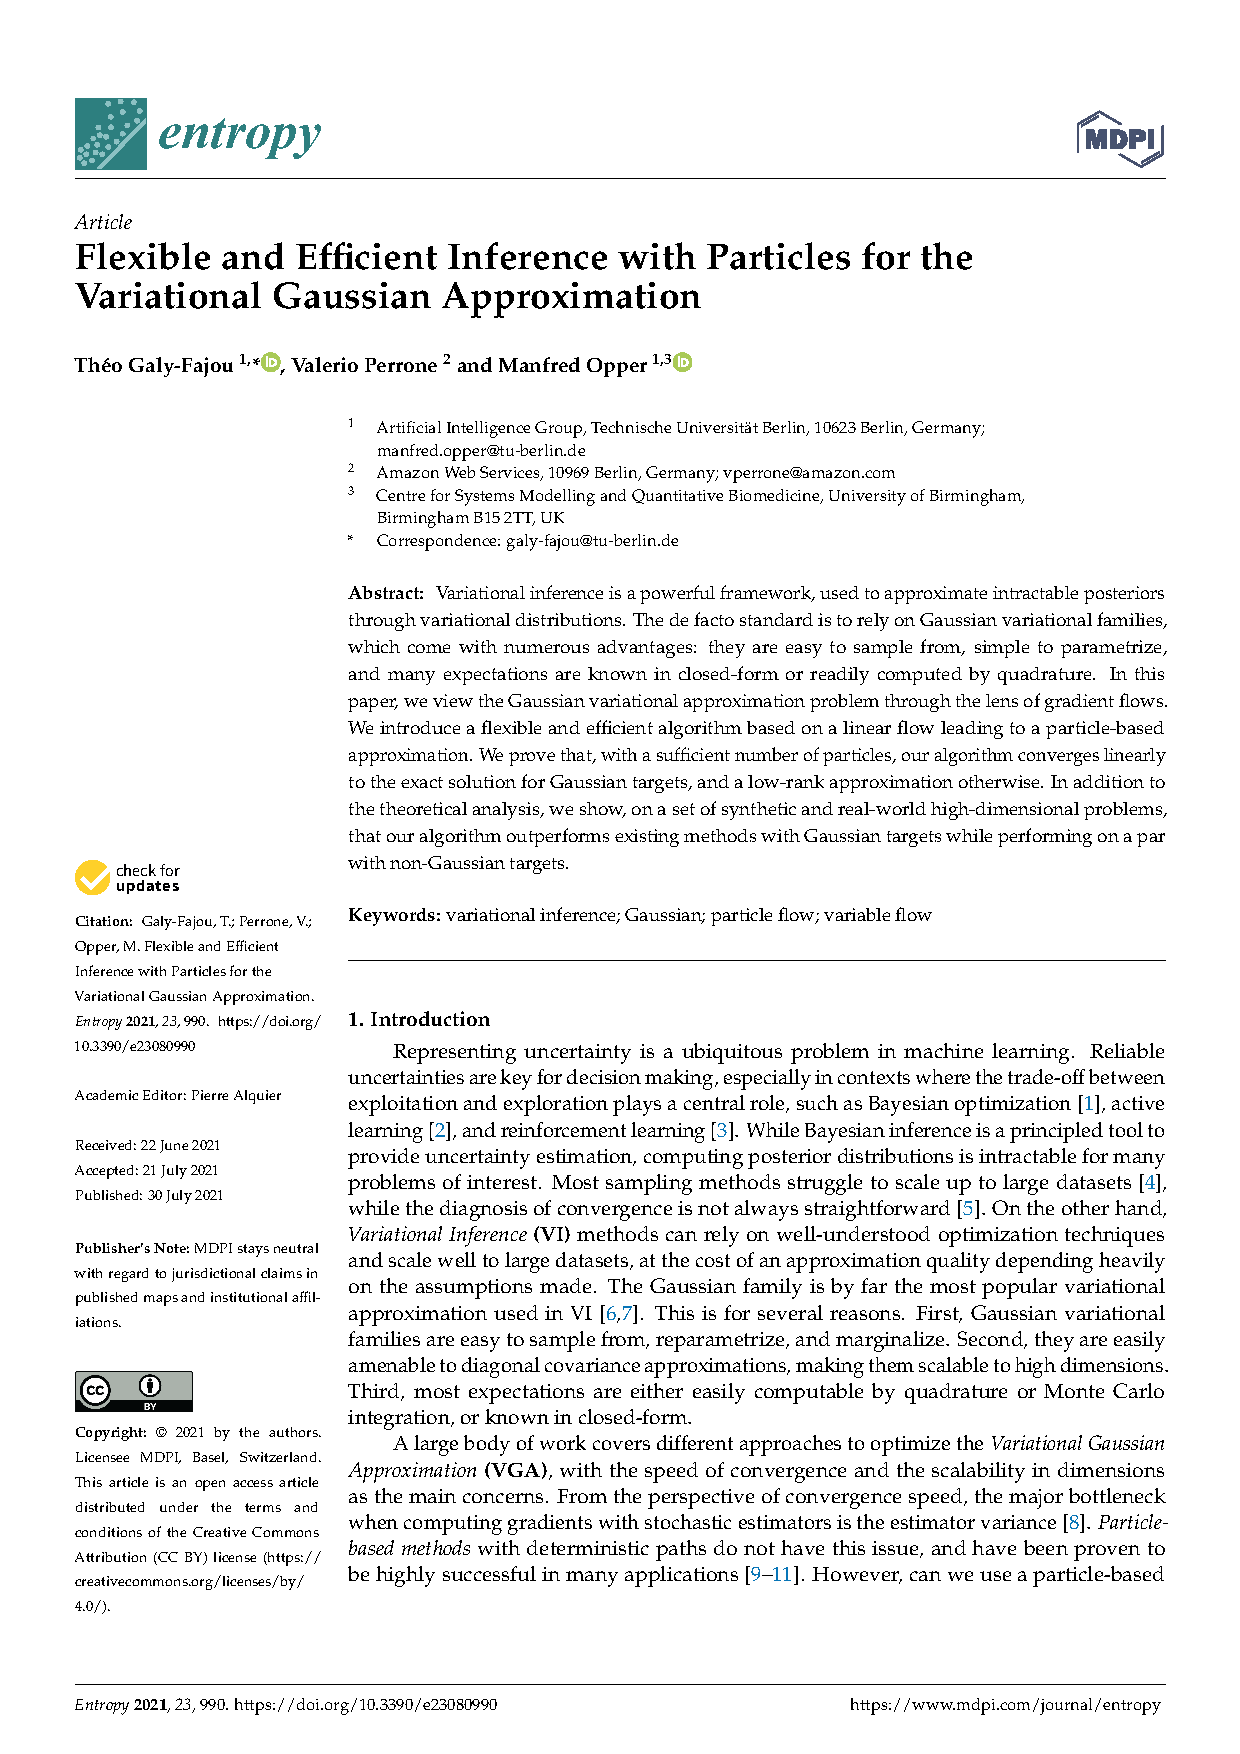
\includepdf[pages=-,pagecommand={},scale=0.95]{./papers/entropy-23-00990-v2.pdf}
% templatesize={\textwidth}{\textheight}
% ---------------------------------------------------------------------------
%: ----------------------- end of thesis sub-document ------------------------
% ---------------------------------------------------------------------------

